\documentclass[12pt, polish, aspectratio = 169]{beamer}
\usepackage{beamer}

\title{Rozprawa Doktorska}
\author{mgr inż. Łukasz Dróżdż}
\subject{Analiza metrologiczna algorytmów dyskretnej transformacji falkowej}
\subtitle{Analiza metrologiczna algorytmów dyskretnej transformacji falkowej}
\institute{Politechnika Śląska, Wydział Elektryczny \\ Katedra Metrologii, Elektroniki i Automatyki}
\keywords{dyskretna transformacja falkowa, cyfrowe przetwarzanie sygnałów, szacowanie niepewności wyniku pomiaru, analiza właściwości metrologicznych toru pomiarowego}

\titlegraphic{
\includegraphics[height = 1cm]{obrazki/polsl_logo}}
\date{Wersja \gitVer{} z \today{}}

\begin{document}

\section*{Wstęp}

\begin{frame}[plain]
\titlepage
\end{frame}

\begin{frame}{Plan prezentacji}
\tableofcontents
\end{frame}

\newsection{Teza pracy}{Przedstawienie tezy pracy oraz jej najważniejszych założeń}

\begin{frame}{Teza pracy}
\justifying
Stosując przedstawiony model błędów oraz zaproponowaną metodę szacowania wypadkowej wartości niepewności rozszerzonej istnieje możliwość oszacowania wartości niepewności rozszerzonych dla wielkości wyjściowych toru pomiarowego wykorzystującego algorytm dyskretnej transformacji falkowej.

Oszacowanie wartości niepewności rozszerzonych dla omawianych wielkości jest możliwe w trakcie działania systemu pomiarowego, również w przypadku zmiany parametrów pracy tego systemu oraz zmiany parametrów modelu błędów.

Skuteczność zaproponowanej metody oraz dokładność uzyskiwanych wyników zależą od dokładności przyjętych parametrów modelu błędów, przy czym uzyskiwane wyniki są zbieżne z uzyskiwanymi metodą Monte-Carlo.
\end{frame}

\begin{frame}{Podsumowanie tezy}
\begin{itemize}
\item Propozycja modelu błędów umożliwiającego opis właściwości metrologicznych torów pomiarowych wykorzystujących algorytmy transformacji falkowej
\item Propozycja metody szacowania wartości wypadkowej niepewności rozszerzonej, która:
	\begin{itemize}
	\item cechuje się niską złożonością obliczeniową i jest możliwa do stosowania w czasie pracy systemu pomiarowego
	\item daje możliwość zmiany parametrów modelu błędów podczas pracy systemu pomiarowego, zachowując niską złożoność obliczeniową
	\end{itemize}
\item Wyniki uzyskiwane przy użyciu zaproponowanej metody powinny być zbieżne z wynikami uzyskiwanymi metodą Monte-Carlo
\item Dokładność uzyskiwanych wyników może zależeć od dokładności wyznaczenia parametrów modelu błędu
\end{itemize}
\end{frame}

\newsection{Algorytm transformacji falkowej}{Przedstawienie najważniejszych właściwości metrologicznych algorytmów transformacji falkowej}

\begin{frame}{Algorytm transformacji falkowej}
\begin{equation}
w_{a,b} = \frac{1}{\sqrt{a}} \int _{-\infty} ^{\infty} x \emb{t} \psi \emb{\frac{t-b}{a}} dt \label{eq:cwt}
\end{equation}
\begin{itemize}
\item Wykorzystuje funkcję \enquote{falki-matki}, oznaczoną jako $\psi(t)$
\item Umożliwia analizę sygnału $x(t)$ w dziedzinie skala-czas
\item Dla wybranej skali $a$ współczynniki transformacji $w_{a,b}$ wyznaczane są dla kolejnych okien pomiarowych, przesuniętych o czas $b$
\item Parametr skali $a$ określa zakres częstotliwości harmonicznych sygnału $x(t)$
\item Występuje w kilku głównych odmianach:
	\begin{itemize}
	\item[CWT] ciągła transformacja falkowa
	\item[DWT] dyskretna transformacja falkowa
	\item[UFWT] dyskretna transformacja falkowa bez decymacji
	\end{itemize}
\end{itemize}
\end{frame}

\begin{frame}{Obszary zastosowań algorytmu}
\begin{itemize}
\item Umożliwiają detekcję, czy zjawisko o określonym widmie częstotliwościowym miało miejsce w danym czasie
\end{itemize}
\begin{itemize}
\item Przetwarzanie, kompresja oraz analiza obrazów i dźwięków
\item Redukcja szumu w sygnale pomiarowym
\item Analiza sygnałów EKG oraz EEG
\item Analiza przebiegu drgań sejsmicznych
\item Bezinwazyjna analiza stanu elementów mechanicznych
\item Algorytmy stratnej kompresji danych
\item Analiza zwarć wysoko prądowych
\item Analiza procesów hydrologicznych
\end{itemize}
\end{frame}

\begin{frame}{Algorytm dyskretnej transformacji falkowej}
\begin{equation}
w_{m,n} = \frac{1}{\sqrt{2^{m}}} \int _{-\infty} ^{\infty} x \emb{t} \psi \emb{\frac{t - n 2^{m}}{2^{m}}} dt \label{eq:dwt}
\end{equation}
\begin{itemize}
\item Wyznaczenie nieskończonej liczby współczynników transformacji jest niemożliwe, a wyznaczanie nadmiarowej liczby współczynników transformacji nie jest konieczne w celu analizy i rekonstrukcji sygnału
\item Wprowadzenie ograniczenia dostępnych wartości dla parametrów skali $a$ oraz przesunięcia w czasie $b$, gdzie $a = 2^m$, $b = n2^m$ dla $m, n \in \mathbb{N}$ zapewnia:
	\begin{itemize}
	\item eliminację nadmiarowych współczynników transformacji $w_{m,n}$
	\item możliwość rekonstrukcji oryginalnego sygnału $x(t)$
	\item dynamiczną rozdzielczość podstawy czasu dla kolejnych skal
	\end{itemize}
\item Symbol $m$ oznacza numer skali (zakres częstotliwości)
\item Symbol $n$ oznacza numer okna pomiarowego
\end{itemize}
\end{frame}

\begin{frame}{Proces dekompozycji sygnału}
\begin{figure}
\includegraphics[scale = 0.75]{obrazki/dwt_dekompozycja}
\caption{Przykład trzech iteracji procesu dekompozycji sygnału}
\label{fig:fwt_decomp}
\end{figure}
\begin{itemize}
\item $S_{0}$ to kolejne próbki przetwarzanego sygnału $x(i)$
\item $S_{m}$ to kolejne próbki aproksymacji sygnału dla skali $m$
\item $T_{m}$ to kolejne próbki detali sygnału dla skali $m$
\end{itemize}
\end{frame}

\begin{frame}{Bank filtrów algorytmu}
\begin{figure}
\includegraphics[scale = 0.75]{obrazki/bank_db_short}
\caption{Przykładowe banki filtrów dla rodziny \enquote{Daubechies}, częstotliwość znormalizowano do połowy częstotliwości próbkowania, wartość wzmocnienia znormalizowano do maksymalnej wartości wzmocnienia dla każdego filtru z osobna}
\end{figure}
\end{frame}

\begin{frame}{Właściwości metrologiczne algorytmu}
\begin{itemize}
\item Algorytm przetwarza sygnały błędów obecne w sygnale wejściowym zgodnie z charakterystyką banku filtrów
\item Rzeczywista implementacja algorytmu wprowadza błędy własne, związane z operacjami arytmetycznymi
\item Proponowane w literaturze metody analizy są skomplikowane, a dodatkowo ich aplikacja w przypadku zmiany parametrów algorytmu wiąże się z powtórnym procesem analizy, co jest czasochłonne
\item Nie zawsze znane są jawne postaci funkcji falki-matki $\psi(t)$ oraz funkcji skalującej $\phi(t)$ dla wybranej rodziny, co utrudnia analizę
\item Projektant toru pomiarowego nie jest zwykle ekspertem z dziedziny falek, a jedynie użytkownikiem stosującym gotową implementację algorytmu
\end{itemize}
\end{frame}

\begin{frame}{Błędy własne algorytmu}
\begin{equation}
e_{X,z} \emb{j} = \tilde{X} \emb{j} - \dot{X} \emb{j} \label{eq:fwt_outerr_self}
\end{equation}
\begin{itemize}
\item Sygnał błędu własnego $e_{X,z}(j)$ związany z $j$-tą wielkością wyjściową wynika z zaokrągleń wykonywanych podczas operacji arytmetycznych
\item Parametry sygnału błędu własnego zaokrągleń powinny być wyznaczane dla rzeczywistej implementacji algorytmu o wybranych parametrach
\item Eksperyment należy przeprowadzić zakładając, że wielkości wejściowe $x(i)$ algorytmu nie są obarczone żadnymi błędami, zatem $\tilde{x}(t) = \dot{x}(t)$
\item Dla algorytmu idealnego sygnał ten nie występuje, wtedy $e_{X,z}(j) = 0$
\end{itemize}
\end{frame}

\begin{frame}{Błędy własne algorytmu}
\begin{figure}
\includegraphics[scale = 0.75]{obrazki/schemat_dwt_ew}
\caption{Schemat blokowy procedury wyznaczania pojedynczej realizacji sygnału błędu własnego $e_{X,z}(j)$ algorytmu transformacji falkowej}
\end{figure}
\end{frame}

\begin{frame}{Wariancja sygnału błędu własnego zaokrągleń}
\begin{figure}
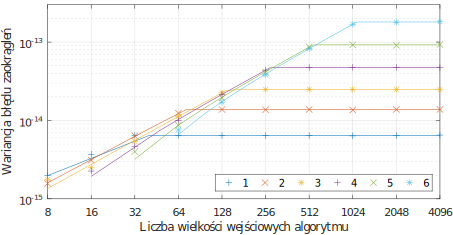
\includegraphics[scale = 0.75]{obrazki/dwt_rerror_coif5}
\caption{Wartość wariancji sygnału błędu $e_{X,z}(j)$ w funkcji wybranych parametrów algorytmu DWT, falka \enquote{coif5}, liczby o długości~\qty{32}{\bitOw}, ostatni etap dekompozycji}
\end{figure}
\end{frame}

\begin{frame}{Wariancja sygnału błędu własnego zaokrągleń}
\begin{itemize}
\item Zależy od liczby przeprowadzanych operacji arytmetycznych, a zatem:
	\begin{itemize}
	\item wzrasta wraz ze wzrostem liczby iteracji procesu dekompozycji sygnału
	\item wzrasta wraz ze wzrostem rzędu falki
	\item wzrasta wraz ze wzrostem liczby wielkości wejściowych
	\end{itemize}
\item Zależy od długości słowa liczb zmiennoprzecinkowych
\item Zależy od zakresu wartości wielkości wejściowych
\item Powinna być wyznaczana w warunkach zbliżonych do warunków pracy rzeczywistego algorytmu
\item Długość słowa należy dobrać tak, aby wariancja sygnału błędu własnego była niewielka w stosunku do wariancji wypadkowego sygnału błędu przetwarzanych wielkości
\end{itemize}
\end{frame}

\newsection{Model błędów}{Omówienie najważniejszych założeń odnośnie zaproponowanego w pracy modelu błędów}

\begin{frame}{Podstawowe założenia modelu błędów}
\begin{itemize}
\item Możliwość analizy sygnałów błędów opisanych deterministycznie i niedeterministycznie
\item Uwzględnienie wpływu widma przetwarzanego sygnału na właściwości metrologiczne toru pomiarowego
\item Sygnał błędu opisany jako różnica pomiędzy idealnym i rzeczywistym przebiegiem analizowanej wielkości
\item Idealny przebieg analizowanej wielkości wynika z założeń odnośnie realizowanego przez tor pomiarowy zadania
\item Każdy fragment toru pomiarowego przetwarza sygnały błędów obecne w sygnale wejściowym oraz wprowadza sygnały błędów własnych
\item Tor pomiarowy może składać się z wielu obiektów przetwarzających ciągły w czasie sygnał lub kolejne próbki sygnału
\end{itemize}
\end{frame}

\begin{frame}{Podział sygnałów błędów}
\begin{itemize}
\item Podział sygnałów błędów ze względu na charakter realizacji:
	\begin{itemize}
	\item \strong{sygnały błędów statycznych}, których wartości realizacji nie zmieniają się dla analizowanej serii pomiarowej
	\item \strong{sygnały błędów dynamicznych}, których wartości realizacji zmieniają się dla analizowanej serii pomiarowej i są opisane deterministycznie
	\item \strong{sygnały błędów statycznych}, których wartości realizacji zmieniają się dla analizowanej serii pomiarowej zgodnie z regułami probabilistycznymi
	\end{itemize}
\item Podział sygnałów błędów ze względu na genezę:
	\begin{itemize}
	\item \strong{sygnały błędów własnych}, wprowadzanie przez analizowany obiekt
	\item \strong{sygnały błędów propagowanych}, przenoszone z wejścia na wyjście obiektu
	\end{itemize}
\item Termin \enquote{seria pomiarowa} odnosi się zwykle do pojedynczego okna pomiarowego lub zbioru próbek, stanowiących wejście dla pojedynczej realizacji algorytmu przetwarzania danych
\end{itemize}
\end{frame}

\begin{frame}{Model błędu toru pomiarowego}
\begin{figure}
\includegraphics[scale = 0.75]{obrazki/schemat_trans}
\caption{Schemat blokowy toru pomiarowego, na który przedstawiono proces wyznaczania wartości realizacji pojedynczej wielkości wyjściowej}
\end{figure}
\begin{itemize}
\item Wielkość fizyczna $s(t)$ jest przetwarzana na wielkość $y(t)$
\item Kolejne próbki wielkości $y(t)$ reprezentowane są przez wielkość $x(i)$
\item Na podstawie wielkości $x(i)$ wyznaczane są wartości wielkości $X(i)$
\end{itemize}
\end{frame}

\begin{frame}{Analizowane fragmenty toru pomiarowego}
\begin{itemize}
\item \strong{Część analogowa}, która przetwarza ciągły w czasie sygnał $s(t)$
\item \strong{Część cyfrowa}, która przetwarza próbki sygnału $y(t_{i})$
\item \strong{Przetwornik analogowo-cyfrowy}:
	\begin{itemize}
	\item zamienia ciągły w czasie sygnał $y(t)$ na jego dyskretną reprezentację $x(i)$
	\item opisywany jako kaskadowe połączenie modelu części analogowej, idealnego kwantyzatora oraz części cyfrowej
	\end{itemize}
\item Każdy fragment toru pomiarowego posiada właściwości:
	\begin{itemize}
	\item \strong{statyczne}, niezależne od widma przetwarzanego sygnału
	\item \strong{dynamiczne}, zależne od widma przetwarzanego sygnału
	\end{itemize}
\item Tor pomiarowy może składać się z wielu obiektów połączonych kaskadowo
\item Tor pomiarowy może dostarczać na wyjściu wiele wielkości wyjściowych
\end{itemize}
\end{frame}

\begin{frame}{Część analogowa toru pomiarowego}
\begin{figure}
\includegraphics[scale = 0.75]{obrazki/schemat_ciagly}
\caption{Model fragmentu części analogowej toru pomiarowego}
\end{figure}
\begin{itemize}
\item Obiekt przetwarza ciągłą w czasie wielkość $s(t)$ na wielkość $y(t)$
\item Właściwości dynamiczne opisuje transmitancja $G_{y}(j\omega)$
\item Właściwości statyczne opisuje funkcja przetwarzania $f_{y}(x)$
\item Przykładem obiektu może być filtr analogowy, przetwornik pomiarowy, wzmacniacz pomiarowy lub układ próbkująco-pamiętający
\end{itemize}
\end{frame}

\begin{frame}{Część analogowa toru pomiarowego}
\begin{itemize}
\item Parametry $G_{y}(j\omega)$ oraz $f_{y}(x)$ mogą być opisane:
	\begin{itemize}
	\item dla warunków idealnych, jako $\dot{G}_{y}(j\omega)$ oraz $\dot{f}_{y}(x)$
	\item dla warunków rzeczywistych, jako $\tilde{G}_{y}(j\omega)$ oraz $\tilde{f}_{y}(x)$
	\end{itemize}
\item Jeżeli rzeczywiste właściwości obiektu odbiegają od idealnych, obiekt wprowadza do sygnału wyjściowego błędy własne
\item Obiekt przetwarza sygnały błędów zawarte w wielkości wejściowej
\item Dla właściwości dynamicznych opisać można wzmocnienie $K_{y}(\omega)$ oraz przesunięcie fazowe $\varphi_{y}(\omega)$ w funkcji pulsacji $\omega$ jako:
\begin{gather}
K_{y} \emb{\omega} = \left| G_{y} \emb{j\omega} \right| =
	\sqrt{\left( \Re \left( G_{y} \emb{j\omega} \right) \right)^{2} +
	\left( \Im \left( G_{y} \emb{j\omega} \right) \right)^{2}}
\label{eq:mid_cont_amp}, \\
\varphi_{y} \emb{\omega} = \arctan \left( \frac{\Im \left( G_{y} \emb{j\omega} \right)}{\Re \left( G_{y} \emb{j\omega} \right)} \right) \label{eq:mid_cont_phi}.
\end{gather}
\end{itemize}
\end{frame}

\begin{frame}{Część analogowa toru pomiarowego}
\begin{itemize}
\item Wielkość wejściowa $s(t)$ w przypadku idealnym opisana równaniem:
\begin{equation}
\dot{s} \emb{t} = \sum _{i = 0} ^{\infty} E_{s,o} \emb{\omega_{i}} \sin \left( \omega_{i} t + \varphi_{s,o} \emb{\omega_{i}} \right) \label{eq:in_cont_omega_ideal}
\end{equation}
\item Wielkość wyjściowa $y(t)$ w przypadku idealnym opisana jako:
\begin{equation}
\dot{y} \emb{t} = \dot{f}_{y} \emb{ \sum _{i = 0} ^{\infty} \dot{K}_{y} \emb{\omega_{i}} E_{s,o} \emb{\omega_{i}} \sin \left( \omega_{i} t + \varphi_{s,o} \emb{\omega_{i}} + \dot{\varphi}_{y} \emb{\omega_{i}} \right) } \label{eq:out_cont_omega_ideal}
\end{equation}
\item $E_{s,o}(\omega)$ jest amplitudą harmonicznej sygnału $\dot{s}(t)$
\item $\varphi_{s,o}(\omega)$ jest fazą harmonicznej sygnału $\dot{s}(t)$
\end{itemize}
\end{frame}

\begin{frame}{Część analogowa toru pomiarowego}
\begin{itemize}
\item Wielkość wejściowa $s(t)$ w przypadku rzeczywistym opisana równaniem:
\begin{equation}
\tilde{s} \emb{t} = \dot{s} \emb{t} + e_{s,r} \emb{t} + \sum _{i = 0} ^{\infty} E_{s,e} \emb{\omega} \sin \left( \omega t + \varphi_{s,e} \emb{\omega} \right) \label{eq:in_cont_omega_real}
\end{equation}
\item Wielkość wyjściowa $y(t)$ w przypadku rzeczywistym opisana jako:
\begin{equation}
\tilde{y} \emb{t} = \tilde{f}_{y} \left( \dot{u} \emb{t} + e_{u,\Sigma} \emb{t} \right) + f_{z} \emb{\mathbf{z} \emb{t}} = \dot{y} \emb{t} + e_{y,\Sigma} \emb{t} \label{eq:out_cont_real_all}
\end{equation}
\item $E_{s,e}(\omega)$ jest amplitudą harmonicznej sygnału błędu wielkości wejściowej
\item $\varphi_{s,e}(\omega)$ jest fazą harmonicznej sygnału błędu wielkości wejściowej
\item $f_{z}(\mathbf{z})$ jest funkcją uwzględniającą wielkości zakłócające $\mathbf{z}(t)$
\item $e_{y,\Sigma}(t)$ jest wypadkowym sygnałem błędu wielkości wyjściowej $y(t)$
\end{itemize}
\end{frame}

\begin{frame}{Parametry sygnałów błędów na wyjściu obiektu}
\begin{itemize}
\item Dla sygnałów błędów propagowanych części związanej z właściwościami dynamicznymi obiektu zachodzi:
\begin{equation}
\sigma_{u}^{2} \emb{\omega} = \tilde{K}_{y}^{2} \emb{\omega} \sigma_{s}^{2} \emb{\omega} \label{eq:mid_cont_var_omega}
\end{equation}
\item $\sigma_{s}^{2}$ jest wariancją sygnału na wejściu obiektu, natomiast $\sigma_{u}^{2}$ wariancją tego sygnału na wyjściu fragmentu związanego z właściwościami dynamicznymi
\item W przypadku sygnałów błędów losowych istnieje możliwość oszacowania średniej wariancji tych sygnałów w zadanym zakresie pulsacji:
\begin{equation}
\sigma_{u,rp}^{2} = \frac{1}{a - b} \int _{b} ^{a} \tilde{K}_{y}^{2} \emb{\omega} \sigma_{s,r}^{2} \emb{\omega} d\omega \label{eq:mid_cont_var_rand},
\end{equation}
\item $\sigma_{u,rp}^{2}$ jest średnią wariancją sygnału $e_{s,r}(t)$ przeniesionego na wyjście fragmentu związanego z właściwościami dynamicznymi dla $\omega \in \interval{b}{a}$
\end{itemize}
\end{frame}

\begin{frame}{Parametry sygnałów błędów na wyjściu obiektu}
\begin{itemize}
\item Wariancję sygnału błędu na wyjściu obiektu opisuje równanie:
\begin{equation}
\sigma_{y}^{2} = \text{Var}\emb{\tilde{f}_{y} \emb{e_{u} \emb{t}}} = E \left[ \left( \tilde{f}_{y} \emb{e_{u} \emb{t}} - E \left[ \tilde{f}_{y} \emb{e_{u} \emb{t}} \right] \right)^2 \right] \label{eq:out_cont_var_function}
\end{equation}
\item $e_{u}(t)$ jest analizowanym sygnałem błędu na wyjściu fragmentu obiektu opisującego jego właściwości dynamiczne
\item Jeżeli funkcja przetwarzania $f_{y}(x)$ jest addytywna (tj. zachodzi $f_{y}(a+b) = f_{y}(a) + f_{y}(b)$) istnieje możliwość stosowania zasady superpozycji i analizy wszystkich składowych sygnału błędu $e_{y,\Sigma}(t)$ z osobna
\item Jeżeli funkcja przetwarzania $f_{y}(x)$ jest liniowa (tj. opisana jest w postaci $f_{y}(x) = s_{y} x + b_{y}$) równanie \eqref{eq:out_cont_var_function} upraszcza się do postaci $\sigma_{y}^{2} = s_{y}^{2} \sigma_{u}^{2}$
\end{itemize}
\end{frame}

\begin{frame}{Parametry sygnałów błędów na wyjściu obiektu}
\begin{itemize}
\item W przypadku liniowej funkcji przetwarzania wariancję sygnału błędu na wyjściu obiektu opisuje równanie:
\begin{equation}
\sigma_{y}^{2} \emb{\omega} = \tilde{s}_{y}^{2} \tilde{K}_{y}^{2} \emb{\omega} \sigma_{s}^{2} \emb{\omega} \label{eq:out_cont_var_omega}
\end{equation}
\item $s_{y}$ jest współczynnikiem kierunkowym równania przetwarzania obiektu
\item Jeżeli rzeczywiste wartości wielkości $s_{y}$, $K_{y}(\omega)$, lub rzeczywista postać funkcji przetwarzania $f_{y}(x)$ nie są znane, należy w obliczeniach przyjąć wartości odpowiednie dla idealnych wielkości
\item Kształt funkcji gęstości prawdopodobieństwa analizowanych sygnałów na wyjściu jest identyczny, jak na wejściu obiektu, w przypadku liniowej transmitancji obiektu i liniowej funkcji przetwarzania
\end{itemize}
\end{frame}

\begin{frame}{Przetwornik analogowo-cyfrowy}
\begin{itemize}
\item Przekształca ciągły sygnał wejściowy $y(t)$ na jego dyskretną reprezentację $x(t_{i})$, gdzie $t_{i}$ jest wybraną wartością czasu
\item Właściwości obiektu opisać można stosując:
	\begin{itemize}
	\item model części analogowej do opisu właściwości układu P/P
	\item model części cyfrowej do opisu właściwości układu A/C
	\end{itemize}
\item W przypadku idealnego przetwornika A/C transmitancja $G_{AC}(j\omega) = 1$
\item Funkcję przetwarzania idealnego układu kwantyzatora opisuje równanie:
\begin{equation}
f_{AC} \emb{x} = n_{q} \emb{x} = \left\lfloor \frac{x}{q} + \num{0.5} \right\rfloor \label{eq:adc_function}
\end{equation}
\item $n_{q}(x)$ jest wartością wyjściową przetwornika dla wartości $x$
\item $q$ jest wartością kwantu przetwornika
\end{itemize}
\end{frame}

\begin{frame}{Przetwornik analogowo-cyfrowy}
\begin{itemize}
\item Wielkość wyjściową przetwornika, wyrażoną w jednostce wielkości wejściowej, opisuje równanie:
\begin{equation}
\breve{u}_{AC} \emb{x} = q f_{AC} \emb{x} = q \left\lfloor \frac{x}{q} + \num{0.5} \right\rfloor \label{eq:adc_output}
\end{equation}
\item Błąd kwantowania wyrazić można w postaci:
\begin{equation}
e_{AC,q} \emb{x} = x - \breve{u}_{AC} \emb{x} = x - q \left\lfloor \frac{x}{q} + \num{0.5} \right\rfloor \label{eq:adc_qerror}
\end{equation}
\item Zakres wartości realizacji błędu kwantowania opisuje relacja:
\begin{equation}
-\frac{q}{2} \le \hat{e}_{AC,q} \emb{x} \le \frac{q}{2} \label{eq:adc_qerrrange}
\end{equation}
\end{itemize}
\end{frame}

\begin{frame}{Przetwornik analogowo-cyfrowy}
\begin{itemize}
\item Funkcja przetwarzania dana równaniem \eqref{eq:adc_function} nie jest addytywna
\item Wartości realizacji sygnału błędu kwantowania mogą być skorelowane z przetwarzanym sygnałem
\item Aby zastosować model błędu opisany w pracy proponuje się przyjąć:
\begin{equation}
f_{AC'} \emb{x} = x \label{eq:adc_simplify}
\end{equation}
\item Sygnał błędu kwantowania, wynikający z postaci funkcji przetwarzania opisanej równaniem \eqref{eq:adc_function}, traktować jako sygnał losowy:
	\begin{itemize}
	\item stosując modelu nieskorelowanego sygnału szumu, o charakterze addytywnym i stałej widmowej gęstości mocy
	\item przyjmując jednakowe prawdopodobieństwo uzyskania każdej z wartości realizacji tego sygnału, co opisano relacją \eqref{eq:adc_output}
	\end{itemize}
\end{itemize}
\end{frame}

\begin{frame}{Przetwornik analogowo-cyfrowy}
\begin{itemize}
\item Z treści równania \eqref{eq:adc_simplify} i przyjętych założeń wynika:
\begin{equation}
\dot{x} \emb{i} = \dot{y} \emb{t_{i}} \label{eq:adc_out_ideal}
\end{equation}
\item $x(i)$ stanowi kolejne próbki sygnału na wyjściu przetwornika
\item $y(t)$ jest sygnałem na wejściu przetwornika
\begin{gather}
\tilde{x} \emb{i} = \dot{x} \emb{i} + e_{x,\Sigma} \emb{i} \label{eq:adc_out_real} \\
e_{x,\Sigma} \emb{i} \cong e_{y,\Sigma} \emb{t_{i}} + e_{x,q} \emb{i} + e_{x,w} \emb{i} \label{eq:adc_out_error}
\end{gather}
\item $e_{x,\Sigma}(i)$ jest wypadkowym sygnałem błędu przetwornika
\item $e_{x,q}(i)$ jest sygnałem związanym z błędem kwantowania
\item $e_{x,w}(i)$ dla rzeczywistego przetwornika jest sygnałem błędu własnego
\end{itemize}
\end{frame}

\begin{frame}{Przetwornik analogowo-cyfrowy}
\begin{itemize}
\item Z uwagi na przyjęte założenia, sygnały błędów na wyjściu przetwornika opisać można jako:
\begin{equation}
e_{x} \emb{i} \cong e_{y} \emb{t_{i}} \label{eq:adc_errout}
\end{equation}
\item Parametry sygnałów błędów na wyjściu przetwornika opisuje zależność:
\begin{equation}
\sigma_{x}^{2} \cong \sigma_{y}^{2} \label{eq:adc_varout}
\end{equation}
\item Przetwarzane sygnały błędów zachowują swoje oryginalne parametry
\item Pomija się korelacje sygnału błędu kwantowania z przetwarzanymi sygnałami
\item W przypadku modelowania właściwości rzeczywistego przetwornika:
	\begin{itemize}
	\item należy określić postać sygnału błędu własnego $e_{x,w}(i)$ wynikającego z właściwości układu P/P i właściwości układu A/C
	\item należy wskazać korelacje tego sygnału z pozostałymi sygnałami przetwarzanymi i wprowadzanymi przez analizowany obiekt
	\end{itemize}
\end{itemize}
\end{frame}

\begin{frame}{Część cyfrowa toru pomiarowego}
\begin{figure}
\includegraphics[scale = 0.75]{obrazki/schemat_dyskretny}
\caption{Model fragmentu części cyfrowej toru pomiarowego}
\end{figure}
\begin{itemize}
\item Obiekt przetwarza kolejne próbki wielkości $x(i)$ na próbki wielkości $X(i)$
\item Właściwości dynamiczne opisuje transmitancja $H_{X}(z)$
\item Właściwości statyczne opisuje funkcja przetwarzania $f_{X}(x)$
\item Przykładem obiektu może być filtr cyfrowy, algorytm korekcji statycznej lub dynamicznej oraz jednopunktowy algorytm przetwarzania danych
\end{itemize}
\end{frame}

\begin{frame}{Część cyfrowa toru pomiarowego}
\begin{itemize}
\item Metoda analizy i opisu właściwości części cyfrowej toru pomiarowego jest identyczna, jak w przypadku części analogowej
\item Transmitancję $G_{X}(j\omega)$ obiektu odpowiednią dla okresu próbkowania $T_{p}$ opisuje równanie:
\begin{equation}
G_{X} \emb{j\omega} = H_{X} \emb{e^{j\omega T_{p}}} \label{eq:trans_disc_tocont}
\end{equation}
\item Parametry związane z fragmentem obiektu opisującym jego właściwości dynamiczne opisują równania:
\begin{gather}
K_{X} \emb{\omega} = \sqrt{\left( \Re \left( H_{X} \emb{e^{j\omega T_{p}}} \right) \right)^{2} + \left( \Im \left( H_{X} \emb{e^{j\omega T_{p}}} \right) \right)^{2}} \label{eq:mid_disc_amp} \\
\varphi_{X} \emb{\omega} = \arctan \left( \frac{\Im \left( H_{X} \emb{e^{j\omega T_{p}}} \right)}{\Re \left( H_{X} \emb{e^{j\omega T_{p}}} \right)} \right) \label{eq:mid_disc_phi}
\end{gather}
\end{itemize}
\end{frame}

\begin{frame}{Algorytm jako fragment toru pomiarowego}
\begin{itemize}
\item Przetwarza $N$ kolejnych próbek wielkości wejściowych $x(j)$ na $M$ próbek wielkości wyjściowych $X(i)$
\item Sygnały związane z kolejnymi wielkościami wyjściowymi modelować można stosując opis zaproponowany dla części cyfrowej toru pomiarowego
\item W przypadku liniowych algorytmów przetwarzania danych, działanie algorytmu przedstawia równanie:
\begin{equation}
\begin{bmatrix}
X \emb{0}   \\
X \emb{1}   \\
\vdots      \\
X \emb{M-1}
\end{bmatrix}
=
\begin{bmatrix}
a_{0, 0}   &   a_{0, 1} &   \cdots   &   a_{0, N-1}      \\
a_{1, 0}   &   \ddots   &            &   a_{1, N-1}      \\
\vdots     &            &   \ddots   &   \vdots          \\
a_{M-1, 0} &   \cdots   &   \cdots   &   a_{M-1, N-1}
\end{bmatrix}
\begin{bmatrix}
x \emb{0}   \\
x \emb{1}   \\
\vdots      \\
x \emb{N-1}
\end{bmatrix}
\label{eq:alg_out_mat}
\end{equation}
\item $a_{i,j}$ to kolejne współczynniki macierzy transformacji algorytmu
\end{itemize}
\end{frame}

\begin{frame}{Algorytm jako fragment toru pomiarowego}
\begin{itemize}
\item Pojedynczą $i$-tą wielkość wyjściową opisuje równanie:
\begin{equation}
X \emb{i} = a_{i, 0} x \emb{0} + \hdots + a_{i, N-1} x \emb{N-1} = \sum _{j = 0} ^{N-1} a_{i,j} x \emb{j} \label{eq:alg_out_single}
\end{equation}
\item Sygnał błędu propagowanego, związany z $i$-tą wielkością wyjściową:
\begin{equation}
e_{X,p} \emb{i} = a_{i, 0} e_{x,\Sigma} \emb{0} + \hdots + a_{i, N-1} e_{x,\Sigma} \emb{N-1} = \sum _{j = 0} ^{N-1} a_{i,j} e_{x,\Sigma} \emb{j} \label{eq:alg_outerr}
\end{equation}
\item Transmitancja związana z $i$-tą wielkością wyjściową wynosi:
\begin{equation}
H_{i} \emb{z} = a_{i, 0} + \hdots + a_{i, N-1} z^{-N+1} = \sum _{k = 0} ^{N-1} a_{i, k} z^{-k} \label{eq:alg_trans_single}
\end{equation}
\end{itemize}
\end{frame}

\begin{frame}{Algorytm jako fragment toru pomiarowego}
\begin{itemize}
\item Wartości współczynników macierzy transformacji mogą być wyznaczane:
	\begin{itemize}
	\item na podstawie znajomości transmitancji algorytmu
	\item na podstawie założeń odnośnie algorytmu
	\item stosując algorytm identyfikacji
	\end{itemize}
\item Identyfikacja wartości elementów macierzy transformacji:
	\begin{itemize}
	\item polega na wyznaczaniu realizacji wektora wielkości wyjściowych algorytmu
	\item odbywa się dla gotowej implementacji algorytmu
	\item struktura numeryczna algorytmu nie musi być znana
	\end{itemize}
\item Dla $n \in \interval{0}{N-1}$ wektor wielkości wejściowych:
\begin{equation}
x \emb{n} =
\begin{cases}
	1 & $gdy$~n = j \\
	0 & $gdy$~n \neq j
\end{cases}
\label{eq:wt_ident}
\end{equation}
\item Odpowiedź algorytmu stanowi $n$-tą kolumnę identyfikowanej macierzy
\end{itemize}
\end{frame}

\begin{frame}{Wariancja sygnałów błędów na wyjściu algorytmu}
\begin{itemize}
\item W przypadku sygnałów błędów statycznych:
\begin{equation}
\sigma_{X,sp}^{2} \emb{i} = \sigma_{x,s}^{2} \left( a_{i, 0} + \hdots + a_{i, N-1} \right)^{2} = \sigma_{x,s}^{2} \left( \sum _{j = 0} ^{N-1} a_{i, j} \right)^{2} \label{eq:alg_outvar_stat}
\end{equation}
\item W przypadku sygnałów błędów dynamicznych:
\begin{equation}
\sigma_{X,dp}^{2} \emb{i, \omega} = \frac{1}{2} E_{x,e}^{2} \emb{\omega} \left| H_{i} \emb{e^{j\omega T_{p}}} \right|^{2} \label{eq:alg_outvar_dyn}
\end{equation}
\item W przypadku sygnałów błędów losowych o stałej widmowej gęstości mocy:
\begin{equation}
\sigma_{rp}^{2} \emb{i} = a_{i, 0}^{2} \sigma_{x,r}^{2} + \hdots + a_{i, N-1}^{2} \sigma_{x,r}^{2} = \sigma_{x,r}^{2} \sum _{j=0} ^{N-1} {a_{i, j}^{2}} \label{eq:alg_outvar_rand}
\end{equation}
\end{itemize}
\end{frame}

\begin{frame}{Model błędów algorytmu}
\begin{itemize}
\item Dla pojedynczej wielkości wyjściowej analiza jest identyczna, jak w przypadku części cyfrowej toru pomiarowego
\item Sygnały na wyjściu algorytmu opisane w postaci:
\begin{gather}
\dot{X} \emb{i} = \sum _{j = 0} ^{N-1} \dot{a}_{i,j} \dot{x} \emb{j} \label{eq:alg_out_ideal} \\
\tilde{X} \emb{i} = \dot{X} \emb{i} + e_{X,\Sigma} \emb{i} \label{eq:alg_out_real} \\
e_{X,\Sigma} \emb{i} = e_{X,w} \emb{i} + e_{X,p} \emb{i} \label{eq:alg_out_err}
\end{gather}
\item $e_{X,\Sigma}(i)$ jest sygnałem błędu wypadkowego
\item $e_{X,w}(i)$ jest sygnałem błędu własnego
\item $e_{X,p}(i)$ jest sygnałem błędu propagowanego
\end{itemize}
\end{frame}

\begin{frame}{Algorytmy transformacji falkowej}
\begin{itemize}
\item Algorytm można przedstawić za pomocą $K+1$ fragmentów części cyfrowej toru pomiarowego, gdzie $K$ oznacza liczbę iteracji procesu dekompozycji sygnału, przy czym dla każdego etapu dekompozycji:
	\begin{itemize}
	\item transmitancja związana ze wszystkimi wielkościami wyjściowymi algorytmu jest identyczna
	\item parametry sygnału błędu własnego zaokrągleń są identyczne
	\item powyższe właściwości dotyczą sytuacji, gdy nie stosuje się okna pomiarowego
	\end{itemize}
\item Przyjmuje się, że transmitancja algorytmu jest idealna, stąd:
	\begin{itemize}
	\item algorytm nie wprowadza sygnałów błędów statycznego i dynamicznego
	\item błędy własne algorytmu wynikają jedynie z operacji na liczbach zmiennoprzecinkowych
	\end{itemize}
\item Dla założeń innych, niż przedstawiono, należy stosować analizę odpowiednią dla części cyfrowej, w której nie stosuje się wskazanych uproszczeń
\end{itemize}
\end{frame}

\newsection{Metoda szacowania wypadkowej wartości niepewności rozszerzonej}{Omówienie zaproponowanej metody szacowania wypadkowej wartości niepewności rozszerzonej}

\begin{frame}{Ilościowy opis niedokładności wyniku pomiaru}
\begin{itemize}
\item Stosując miarę niepewności standardowej lub wariancji:
	\begin{itemize}
	\item możliwość powiązania wartości wariancji z mocą sygnału błędu
	\item niewielki stopień skomplikowania obliczeń w przypadku wyznaczania parametrów wypadkowych dla sumy sygnałów błędów
	\item nie zawsze istnieje możliwość wskazania, w jakim przedziale i z jakim prawdopodobieństwem znajdują się wartości realizacji sygnału błędu 
	\end{itemize}
\item Stosując miarę niepewności rozszerzonej:
	\begin{itemize}
	\item możliwość powiązania wartości niepewności standardowej z rozszerzoną dla sygnałów o typowych kształtach funkcji gęstości prawdopodobieństwa wartości realizacji tych sygnałów (współczynnik rozszerzenia)
	\item możliwość wskazania przedziału, w jakim z określonym prawdopodobieństwem znajdują się wartości realizacji sygnału błędu
	\item wysoki stopień skomplikowania obliczeń w przypadku wyznaczania parametrów wypadkowego sygnału błędu
	\end{itemize}
\end{itemize}
\end{frame}

\begin{frame}{Ilościowy opis niedokładności wyniku pomiaru}
\begin{itemize}
\item Dla każdego sygnału błędu należy określić:
	\begin{itemize}
	\item kształt funkcji gęstości prawdopodobieństwa
	\item widmową gęstość mocy
	\item korelacje z pozostałymi sygnałami
	\item rodzaj sygnału na podstawie charakteru realizacji tego sygnału
	\item wartość niepewności rozszerzonej dla jednakowego poziomu ufności
	\end{itemize}
\item W przypadku sygnałów błędów dynamicznych:
	\begin{itemize}
	\item wskazać wypadkowe wartości amplitudy i fazy sygnałów o tej samej pulsacji
	\item parametry wypadkowe wyznaczać tylko dla ostatniego etapu analizy
	\end{itemize}
\end{itemize}
\end{frame}

\begin{frame}{Parametry sygnałów o charakterze deterministycznym}
\begin{itemize}
\item Dla sygnałów opisanych zgodnie z równaniem:
\begin{equation}
e_{i} \emb{t} = E_{i} \sin \left( \omega_{i} t + \varphi_{i} \right) \label{eq:dyn_harm}
\end{equation}
\item Wartość wariancji może być wyznaczana w postaci:
\begin{equation}
\sigma_{i}^{2} = \frac{E_{i}^{2}}{2} \label{eq:dyn_var}
\end{equation}
\item Wartość współczynnika korelacji Pearsona wynosi:
\begin{equation}
r_{i,j} =
\begin{cases}
\cos \left( \varphi_{j} - \varphi_{i} \right) & $dla $ \omega_{i} = \omega_{j} \\
0                                             & $dla $ \omega_{i} \ne \omega_{j}
\end{cases}
\label{eq:dyn_corr}
\end{equation}
\end{itemize}
\end{frame}

\begin{frame}{Parametry sygnałów o charakterze deterministycznym}
\begin{itemize}
\item W przypadku wielu harmonicznych sygnału błędu dynamicznego o jednakowej pulsacji:
\begin{gather}
\mathbf{e}_{i} =
\begin{bmatrix}
e_{i,a} & e_{i,b}
\end{bmatrix}
=
\begin{bmatrix}
E_{i} \cos \emb{\varphi_{i}} & E_{i} \sin \emb{\varphi_{i}}
\end{bmatrix}
\label{eq:dyn_vect}, \\
\mathbf{e}_{\Sigma} =
\begin{bmatrix}
e_{\Sigma,a} & e_{\Sigma,b}
\end{bmatrix}
=
\begin{bmatrix}
\sum _{i = 0} ^{N-1} e_{i,a} & \sum _{i = 0} ^{N-1} e_{i,b}
\end{bmatrix}
\label{eq:dyn_vect_sum} \\
E_{\Sigma} = \sqrt{e_{\Sigma,a}^{2} + e_{\Sigma,b}^{2}} \label{eq:dyn_vect_amp} \\
\varphi_{\Sigma} = \arctan \emb{\frac{e_{\Sigma,b}}{e_{\Sigma,a}}} \label{eq:dyn_vect_phi}
\end{gather}
\item Wyznaczenie wypadkowych parametrów dla harmonicznych o jednakowej pulsacji znacznie upraszcza analizę
\end{itemize}
\end{frame}

\begin{frame}{Wyznaczanie parametrów wypadkowego sygnału błędu}
\begin{itemize}
\item Definiując wypadkowy sygnał błędu w postaci:
\begin{equation}
e_{\Sigma} \emb{t} = e_{0} \emb{t} + e_{1} \emb{t} + \hdots + e_{N-1} \emb{t} \label{eq:err_sum}
\end{equation}
\item Wariancja tego sygnału wynosi:
\begin{equation}
\sigma_{\Sigma}^{2} =
\begin{bmatrix}
\sigma_{0} \\ \sigma_{1} \\ \vdots \\ \sigma_{N-1}
\end{bmatrix}^{T}
\begin{bmatrix}
1         & r_{0,1} & \cdots & r_{0,N-1} \\
r_{1,0}   & 1       &        & r_{1,N-1} \\
\vdots    &         & \ddots & \vdots    \\
r_{N-1,0} & \cdots  & \cdots & 1
\end{bmatrix}
\begin{bmatrix}
\sigma_{0} \\ \sigma_{1} \\ \vdots \\ \sigma_{N-1}
\end{bmatrix}
\label{eq:var_matrix}
\end{equation}
\item Wartości współczynnika korelacji Pearsona wynoszą kolejno:
\begin{equation}
r_{i,j} = r_{j,i} = \frac{\sigma_{i,j}^{2} - \sigma_{i}^{2} - \sigma_{j}^{2}}{2 \sigma_{i} \sigma_{j}} \label{eq:var_corr}
\end{equation}
\end{itemize}
\end{frame}

\begin{frame}{Nipewność rozszerzona wypadkowego sygnału błędu}
\begin{itemize}
\item Jeżeli spełnione zostały warunki centralnego twierdzenia granicznego:
\begin{equation}
U_{\Sigma} = c_{n} \sigma_{\Sigma} \label{eq:unc_sum}
\end{equation}
\item $c_{n}$ jest współczynnikiem rozszerzenia dla poziomu ufności $\alpha$
\item Wyniki są nieprawidłowe, jeśli przyjęto błędne założenia
\end{itemize}
\begin{itemize}
\item W pozostałych przypadkach:
	\begin{itemize}
	\item symulacja metodą Monte-Carlo
	\item metoda propagacji dystrybuant
	\item metoda rozszerzonej reguły kombinacji niepewności
	\item metoda bazująca na zbiorach rozmytych
	\item zastosowanie redukcyjnej arytmetyki interwałowej
	\end{itemize}
\end{itemize}
\end{frame}

\begin{frame}{Metoda redukcyjnej arytmetyki interwałowej}
\begin{equation}
U_{\Sigma} = \sqrt{
\begin{bmatrix}
U_{0} \\ U_{1} \\ \vdots \\ U_{N-1}
\end{bmatrix}^{T}
\begin{bmatrix}
1         & h_{0,1} & \cdots & h_{0,N-1} \\
h_{1,0}   & 1       &        & h_{1,N-1} \\
\vdots    &         & \ddots & \vdots    \\
h_{N-1,0} & \cdots  & \cdots & 1
\end{bmatrix}
\begin{bmatrix}
U_{0} \\ U_{1} \\ \vdots \\ U_{N-1}
\end{bmatrix}}
\label{eq:unc_matrix}
\end{equation}
\begin{itemize}
\item $h_{i,j} = h_{j,i}$ to współczynnik koherencji dla pary sygnałów $e_{i}(t)$ oraz $e_{j}(t)$
\item Metoda wymaga wyznaczenia wartości współczynników koherencji:
	\begin{itemize}
	\item stosując metodę analityczną lub symulacyjną -- nie jest uniwersalna
	\item szacując ich wartości -- wyniki mogą być niedokładne
	\end{itemize}
\item Wartość współczynnika koherencji zależy od parametrów wszystkich analizowanych sygnałów
\end{itemize}
\end{frame}

\begin{frame}{Przypadek dla dwóch sygnałów}
\begin{gather}
U_{a,b} = \sqrt{
\begin{bmatrix}
U_{a} \\ U_{b}
\end{bmatrix}^{T}
\begin{bmatrix}
1         & h_{a,b} \\
h_{b,a}   & 1       \\
\end{bmatrix}
\begin{bmatrix}
U_{a} \\ U_{b}
\end{bmatrix}} =
\sqrt{U_{a}^{2} + U_{b}^{2} + 2 U_{a} U_{b} h_{a,b}}
\label{eq:unc_mattwo} \\
h_{a,b} = h_{b,a} = \frac{U_{a,b}^{2} - U_{a}^{2} - U_{b}^{2}}{2 U_{a} U_{b}} \label{eq:unc_cohertwo}
\end{gather}
\begin{itemize}
\item Wartość współczynnika $h_{a,b} = h_{b,a}$ zmienia się w przypadku zmiany:
	\begin{itemize}
	\item parametrów funkcji gęstości prawdopodobieństwa rozkładu realizacji sygnałów $e_{a}(t)$, $e_{b}(t)$
	\item wartości współczynnika korelacji Pearsona analizowanych sygnałów
	\item wartości niepewności rozszerzonych $U_{a}$ oraz $U_{b}$
	\end{itemize}
\end{itemize}
\end{frame}

\begin{frame}{Aplikacja omawianej metody}
\begin{itemize}
\item Wartości współczynników kształtu wyznaczane na podstawie równania:
\begin{equation}
s_{a,b} = s_{b,a} = \frac{U_{a,b}^{2} - U_{a}^{2} - U_{b}^{2}}{2 U_{a} U_{b}} = \frac{U^{2}}{2 U_{a,b}} - 1 \label{eq:unc_shapertwo}
\end{equation}
\item Korekta wynikająca z centralnego twierdzenie granicznego:
\begin{equation}
k_{i,j} = k_{j,i} = \frac{U_{i}^{2} + U_{j}^{2}}{\sum _{k = 0} ^{N-1} U_{k}^{2}} \label{eq:unc_cohercorrb}
\end{equation}
\item Korekta wynikająca z dysproporcji wartości niepewności rozszerzonych:
\begin{equation}
p_{a,b} = p_{b,a} = \sqrt{\frac{\min \emb{U_{a}, U_{b}}}{\max \emb{U_{a}, U_{b}}}} \label{eq:unc_cohercorra}
\end{equation}
\end{itemize}
\end{frame}

\begin{frame}{Aplikacja omawianej metody}
\begin{itemize}
\item Wartości współczynników koherencji szacowane zgodnie z równaniem:
\begin{equation}
h_{i,j} = h_{j,i} = s_{i,j} p_{i,j} k_{i,j} = s_{i,j} \sqrt{\frac{\min \emb{U_{i}, U_{j}}}{\max \emb{U_{i}, U_{j}}}} \left( \frac{U_{i}^{2} + U_{j}^{2}}{\sum _{k = 0} ^{N-1} U_{k}^{2}} \right) \label{eq:unc_coher}
\end{equation}
\item W celu aplikacji metody należy:
	\begin{itemize}
	\item wyznaczyć wartości współczynników kształtu -- operacja jednorazowa
	\item skorygować wartości współczynników kształtu dla obecnych parametrów
	\item zastosować równanie \eqref{eq:unc_matrix} dla uzyskanych wartości
	\end{itemize}
\item Najistotniejsze cechy metody:
	\begin{itemize}
	\item niska złożoność obliczeniowa -- możliwość stosowania w czasie rzeczywistym
	\item możliwość zmiany parametrów modelu błędów
	\item wartości niepewności rozszerzonej szacowane z dokładnością \qty{\pm 5}{\percent}
	\end{itemize}
\end{itemize}
\end{frame}

\newsection{Weryfikacja przedstawionej tezy}{Przedstawienie wyników badań symulacyjnych i pomiarowych, weryfikujących zasadność tezy pracy}

\begin{frame}{Symulacyjna weryfikacja tezy}
\begin{figure}
\includegraphics[scale = 0.75]{obrazki/schemat_symul}
\caption{Schemat blokowy toru pomiarowego będącego obiektem eksperymentu symulacyjnego}
\label{fig:chain_symul}
\end{figure}
\begin{itemize}
\item $s(t)$ to fizyczna, zmienna w czasie wielkość wejściowa
\item $y_{a}(t)$ to napięciowa reprezentacja wielkości mierzonej
\item $y_{b}(t)$ to wielkość wejściowa przetwornika A/C z wbudowanym układem P/P
\item $x_{c}(t)$ to dyskretna reprezentacja wielkości $s(t)$
\item $X(k)$ to kolejne wielkości wyjściowe wyznaczane dla $j$-tej realizacji pomiaru
\end{itemize}
\end{frame}

\begin{frame}{Założenia eksperymentu symulacyjnego}
\begin{gather}
\dot{s} \emb{t} = \frac{6}{10} \sin \left( 2 \pi f_{1} t \right) - \frac{3}{10} \sin \left( 10 \pi f_{1} t + \frac{\pi}{8} \right) + \frac{1}{10} \sin \left( 30 \pi f_{1} t + \frac{\pi}{6} \right) \label{eq:sym_in_ideal} \\
\tilde{s} \emb{t} = \dot{s} \emb{t} + e_{s,r} \emb{t} = e_{s,r} \emb{t} + \sum _{i=1} ^{3} E_{s,o} \emb{\omega_{s,i}} \sin \emb{\omega_{s,i} t + \varphi_{s,i}} \label{eq:sym_in_real}
\end{gather}
\begin{itemize}
\item Częstotliwość podstawowej harmonicznej sygnału $s(t)$ wynosi $f_{1} = \qty{1}{kHz}$
\item Częstotliwość próbkowania wynosi $f_{s} = \qty{48}{kHz}$
\item Algorytm DWT przetwarza $N=8$ próbek wielkości wejściowych na $M=8$ próbek wielkości wyjściowych stosując falkę \enquote{db4} dla dwóch iteracji procesu dekompozycji sygnału
\end{itemize}
\end{frame}

\begin{frame}{Założenia eksperymentu symulacyjnego}
\begin{itemize}
\item Sygnał $s(t)$ jest zakłócony sygnałem szumu białego $e_{s,r}(t)$
\item Przetwornik pomiarowy wprowadza błąd związany z nieliniowością
\item Temperatura otoczenia ma wpływ na dryft zera wzmacniacza i przetwornika pomiarowego, natomiast nie jest ona mierzona
\item Właściwości dynamiczne przetwornika oraz wzmacniacza pomiarowego są nieidealne i opisują je parametry częstotliwości granicznej
\item Przetwornik A/C wprowadza błąd związany z kwantowaniem, natomiast układ P/P jest idealny
\item Algorytm DWT wprowadza błąd związany z operacjami arytmetycznymi
\end{itemize}
\end{frame}

\begin{frame}{Analiza właściwości metrologicznych toru pomiarowego}
\begin{itemize}
\item Na podstawie właściwości każdego z obiektów określono:
	\begin{itemize}
	\item idealne oraz rzeczywiste parametry transmitancji i funkcji przetwarzania
	\item parametry sygnałów błędów wprowadzane przez obiekt
	\item wpływ obiektu na parametry przetwarzanych sygnałów błędów
	\end{itemize}
\item Dla każdego fragmentu toru pomiarowego określono budżet niepewności:
	\begin{itemize}
	\item wskazujący wypadkowe parametry dla analizowanych grup sygnałów błędów
	\item wskazujący parametry wszystkich sygnałów błędów z osobna
	\end{itemize}
\item Dla każdej wielkości wyprowadzano odpowiednie zależności na podstawie wynikających z przyjętego modelu błędu założeń
\item Podczas analizy wyznaczano wartości wybranych wielkości w celu weryfikacji poprawności stosowanej metody
\end{itemize}
\end{frame}

\begin{frame}{Analiza właściwości metrologicznych toru pomiarowego}
\begin{itemize}
\item Dla każdej wielkości wyjściowej wyznaczano niepewności rozszerzone:
	\begin{itemize}
	\item $U_{a}$ zakładając, że spełnione są warunki centralnego twierdzenia granicznego
	\item $U_{b}$ stosując zaproponowaną metodę dla budżetu niepewności uwzględniającego wypadkowe parametry sygnałów błędów
	\item $U_{c}$ stosując zaproponowaną metodę dla budżetu niepewności uwzględniającego wszystkie sygnały błędów z osobna
	\item $U_{d}$ wyznaczone dla budżetu niepewności stosowanego dla $U_{c}$, natomiast bez uwzględniania korekty opisanej równaniem \eqref{eq:unc_cohercorrb}
	\item $U_{s}$ wykonując symulację metodą Monte-Carlo
	\end{itemize}
\item Dla każdej wielkości wyjściowej wyznaczano wariancję sygnału błędu:
	\begin{itemize}
	\item $\sigma^{2}_{ab}$ zgodnie z równaniem \eqref{eq:var_matrix}
	\item $\sigma^{2}_{s}$ stosując metodę Monte-Carlo
	\end{itemize}
\end{itemize}
\end{frame}

\begin{frame}{Analiza właściwości metrologicznych toru pomiarowego}
\begin{itemize}
\item Wartości $U_{*}$ uzyskane analitycznie porównywano z wartościami $U_{s}$ uzyskanymi metodą Monte-Carlo
\item Względny błąd oszacowania wartości niepewności rozszerzonej wynosił:
\begin{equation}
\delta_{U} = 100 \frac{U_{*} - U_{s}}{U_{s}}~\unit{\percent} \label{eq:unc_error}
\end{equation}
\item Wartość współczynnika rozszerzenia szacowano zgodnie z równaniem:
\begin{equation}
c_{*} = \frac{U_{*}}{\sigma_{ab}} \label{eq:unc_coverfact}
\end{equation}
\end{itemize}
\end{frame}

\begin{frame}{Wyniki eksperymentu}
\begin{table}
\begin{center}
\caption{Wyniki przeprowadzonego eksperymentu symulacyjnego}
\footnotesize
\label{tab:sym_partd_params_unc_sum_b}
\begin{tabular}[c]{| c *{5}{|S[table-format = 2.2]} *{4}{|S[table-format = +1.2]} |} \hline
\multirow{2}{*}{\textbf{Wielkość}} & \multicolumn{5}{c|}{\textbf{Niepewność, mV}} & \multicolumn{4}{c|}{\textbf{Błąd, \%}} \\ \cline{2-10}
& $U_{a}$ & $U_{b}$ & $U_{c}$ & $U_{d}$ & $U_{s}$ & $\delta_{a}$ & $\delta_{b}$ & $\delta_{c}$ & $\delta_{d}$ \\ \hline
$S_{2,0}$ & 75.01 & 74.00 & 74.10 & 77.32 & 72.87 & +2.94 & +1.55 & +1.69 & +6.11 \\ \hline
$S_{2,1}$ & 68.19 & 68.44 & 68.43 & 71.52 & 67.09 & +1.64 & +2.01 & +2.00 & +6.60 \\ \hline
$T_{2,0}$ & 57.29 & 56.26 & 55.91 & 57.58 & 53.89 & +6.31 & +4.40 & +3.75 & +6.85 \\ \hline
$T_{2,1}$ & 58.86 & 55.59 & 55.60 & 59.47 & 54.92 & +7.17 & +1.22 & +1.24 & +8.28 \\ \hline
$T_{1,0}$ & 47.31 & 43.61 & 43.37 & 46.09 & 43.76 & +8.11 & -0.34 & -0.89 & +5.32 \\ \hline
$T_{1,1}$ & 47.31 & 43.60 & 43.37 & 46.08 & 43.74 & +8.16 & -0.32 & -0.85 & +5.35 \\ \hline
$T_{1,2}$ & 47.31 & 43.60 & 43.37 & 46.08 & 43.76 & +8.11 & -0.37 & -0.89 & +5.30 \\ \hline
$T_{1,3}$ & 44.79 & 43.64 & 43.39 & 45.43 & 43.17 & +3.75 & +1.09 & +0.51 & +5.24 \\ \hline
\end{tabular}
\end{center}
\end{table}
\end{frame}

\begin{frame}{Pomiarowa weryfikacja tezy}
\begin{figure}
\includegraphics[scale = 0.75]{obrazki/schemat_real}
\caption{Schemat blokowy toru pomiarowego będącego obiektem eksperymentu pomiarowego}
\label{fig:chain_real}
\end{figure}
\begin{itemize}
\item $s(t)$ to zmienne w czasie napięcie mierzone
\item $x(i)$ to wyrażona w jednostce $s(t)$ dyskretna reprezentacja tej wielkości
\item $\mathbf{X}(j)$ to wektory wielkości wyjściowych dla $j$-tej realizacji pomiaru
\end{itemize}
\end{frame}

\begin{frame}{Założenia eksperymentu pomiarowego}
\begin{itemize}
\item Sygnał $s(t)$ pochodził z generatora RIGOL DG1011, gdzie stosowano:
	\begin{itemize}
	\item przebieg sinusoidalny
	\item przebieg trójkątny
	\end{itemize}
\item Dla sygnału $s(t)$ stosowano model błędów uwzględniający parametry generatora oraz syntezowanego sygnału
\item Parametry toru pomiarowego identyfikowano pomiarowo lub szacowano na podstawie dokumentacji fragmentów tego toru
\item Temperatura była stała i wynosiła \qty{21}{\degreeCelsius}
\item Częstotliwość próbkowania sygnału wynosiła $f_{s} = \qty{48}{kHz}$
\item Tor pomiarowy pobierał $N=128$ próbek wielkości wejściowych i wyznaczał na ich podstawie $M=128$ próbek wielkości wyjściowych
\item Dla algorytmu DWT stosowano falkę \enquote{spline4:4} oraz pięć iteracji procesu dekompozycji sygnału
\end{itemize}
\end{frame}

\begin{frame}{Identyfikacja właściwości toru pomiarowego}
\begin{itemize}
\item Właściwości dynamiczne wzmacniacza pomiarowego:
	\begin{itemize}
	\item zidentyfikowano pomiarowo stosując generator RIGOL DG1011 oraz oscyloskop DS5062MA
	\item mierzono przesunięcie fazowe oraz wzmocnienie dla sygnału sinusoidalnego
	\item charakterystykę fazową aproksymowano wielomianem
	\item przyjęto stałe wzmocnienie dla częstotliwości $\hat{f} \in \interval{0}{f_{s}}$
	\item dla filtru RC znajdującego się na wyjściu wzmacniacza zastosowano model wynikający z parametrów filtru
	\end{itemize}
\item Właściwości dynamiczne układu A/C oraz P/P:
	\begin{itemize}
	\item zastosowano model filtru RC pierwszego rzędu
	\item parametry filtru przyjęto zgodnie z dokumentacją 
	\end{itemize}
\item Właściwości statyczne fragmentu przetwarzającego $s(t)$ na $x(i)$:
	\begin{itemize}
	\item zweryfikowano pomiarowo stosując kalibrator FLUKE 5700A
	\item zidentyfikowane sygnały błędów zaliczono do sygnałów błędów losowych
	\end{itemize}
\end{itemize}
\end{frame}

\begin{frame}{Właściwości statyczne toru pomiarowego}
\begin{figure}
\begin{center}
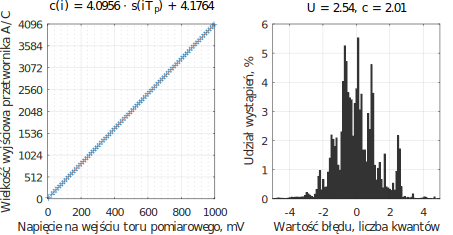
\includegraphics[scale = 0.75]{obrazki/static_adcout}
\caption{Zależność wartości wielkości wyjściowej przetwornika analogowo-cyfrowego w funkcji wartości napięcia wejściowego analizowanego toru pomiarowego oraz histogram uzyskanych realizacji błędu losowego wielkości wyjściowej $c(i)$ przetwornika analogowo-cyfrowego}
\label{fig:pom_static_fun}
\end{center}
\end{figure}
\end{frame}

\begin{frame}{Właściwości statyczne toru pomiarowego}
\begin{gather}
\overline{c} \emb{k} = f_{c} \emb{f_{y} \emb{\hat{s} \emb{k}}} \approx \num{4097.96} \cdot \hat{s} \emb{k} + \num{3.519} \label{eq:pom_func_static} \\
\overline{x} \emb{k} = f_{x} \emb{\overline{c} \emb{k}} = f_{x} \emb{f_{c} \emb{f_{y} \emb{\hat{s} \emb{k}}}} = \frac{\overline{c} \emb{k} - \num{3.519}}{\num{4097.96}} \approx \hat{s} \emb{k} \label{eq:pom_funx_static}
\end{gather}
\begin{itemize}
\item $\overline{c}(k)$ to średnia wartości realizacji sygnału $c(i)$ dla $k$-tej serii pomiarowej
\item $\overline{x}(k)$ to średnia wartości realizacji sygnału $x(i)$ dla $k$-tej serii pomiarowej
\item Dla $k$-tej serii pomiarowej stosowano stałą wartość wielkości $\hat{s}(t)$
\item Sygnał błędu $e_{x,rw}(i)$ jest związany z właściwościami statycznymi obiektu
	\begin{itemize}
	\item na podstawie wykonanych pomiarów przyjęto $U_{x,rw} = \qty{0.38}{mV}$
	\item założono model sygnału zgodny z modelem addytywnego szumu białego
	\item sygnał uwzględnia wszystkie źródła błędów dla właściwości statycznych
	\end{itemize}
\end{itemize}
\end{frame}

\begin{frame}{Właściwości dynamiczne wzmacniacza pomiarowego}
\begin{figure}
\begin{center}
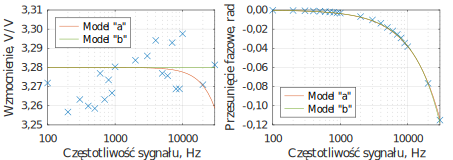
\includegraphics[scale = 0.75]{obrazki/dynamic_ampout}
\caption{Zależność wartości wzmocnienia oraz przesunięcia fazowego w funkcji częstotliwości dla zastosowanej konfiguracji wzmacniacza pomiarowego}
\label{fig:pom_dynamic_ampout}
\end{center}
\end{figure}
\end{frame}

\begin{frame}{Właściwości dynamiczne wzmacniacza pomiarowego}
\begin{gather}
\tilde{K}_{s,x} \emb{\omega} = \tilde{K}_{y} \emb{\omega} \tilde{K}_{c} \emb{\omega} \tilde{K}_{x} \emb{\omega} \label{eq:pom_dwtin_amp} \\
\tilde{K}_{s,x} \emb{\omega} \approx \dot{K}_{s,x} \emb{\omega} = \qty{1}{V \per V} \label{eq:pom_dwtin_ampideal} \\
\tilde{\varphi}_{s,x} \emb{\omega} = \tilde{\varphi}_{y} \emb{\omega} + \tilde{\varphi}_{s,x} \emb{\omega} \approx -\frac{\num{6.82}}{\num{e13}} \omega^{2} - \frac{\num{5.46}}{\num{e07}} \omega - \arctan \emb{\frac{\num{6.69}}{\num{e9}} \omega} \label{eq:pom_dwtin_phi} \\
\dot{\varphi}_{s,x}(\omega) = \qty{0}{rad} \label{eq:pom_dwtin_phiideal}
\end{gather}
\begin{itemize}
\item $K_{s,x}(\omega)$ jest wzmocnieniem sygnału $x(i)$ w stosunku do sygnału $s(t)$
\item $\varphi_{s,x}(\omega)$ jest przesunięciem sygnału $x(i)$ w stosunku do sygnału $s(t)$
\end{itemize}
\end{frame}

\begin{frame}{Zdefiniowane sygnały błędów}
\begin{itemize}
\item $e_{x,rw}(i)$ -- losowy własny, zidentyfikowane właściwości statyczne
\item $e_{x,dw}(i)$ -- dynamiczny własny, zidentyfikowane właściwości dynamiczne
\item $e_{x,dp}(i)$ -- dynamiczny propagowany, sygnał błędu dynamicznego w $s(t)$
\item $e_{x,sp}(i)$ -- statyczny propagowany, sygnał błędu statycznego w $s(t)$
\item $e_{x,rp}(i)$ -- losowy propagowany, sygnał szumu wielkości $s(t)$
\end{itemize}
\begin{itemize}
\item Rzeczywiste parametry sygnału $s(t)$ weryfikowano stosując multimetr Agilent 3458A lub pozostawiano nieznane
\item W przypadku, gdy znane są rzeczywiste parametry sygnału $s(t)$ zachodzi $e_{x,dp}(i) = e_{x,sp}(i) = 0$
\item Dla nieznanych wartości parametrów sygnału $s(t)$ definiowano sygnały błędów obecne w tym sygnale na podstawie dokumentacji generatora
\end{itemize}
\end{frame}

\begin{frame}{Pomiarowa weryfikacja tezy}
\begin{itemize}
\item Na wejście toru pomiarowego podawano sygnał sinusoidalny/trójkątny o zadanych parametrach
\item Parametry sygnału weryfikowano multimetrem Agilent 3458A lub pozostawiano nieznane
\item Wyjście synchronizujące generatora wykorzystywano do ustalania fazy początkowej $\hat{t}_{0}$ sygnału $s(t+\hat{t}_{0})$
\item Dla losowej wartości fazy pobierano wektor realizacji wielkości wejściowych
\item Wyznaczano wartości wielkości wyjściowych algorytmu
\item Na podstawie modelu matematycznego syntezowanego sygnału w przypadku idealnym wyznaczano idealne wartości realizacji wektorów wielkości wejściowych i wyjściowych
\item Powtarzając eksperyment \num{30000} razy wyznaczano niepewności rozszerzone dla wielkości wejściowych i wyjściowych algorytmu DWT
\end{itemize}
\end{frame}

\begin{frame}{Przypadek sygnału monoharmonicznego}
\begin{figure}
\begin{center}
\includegraphics[scale = 0.75]{obrazki/sinfit_error}
\caption{Zależność wartości względnego błędu oszacowania wartości niepewności rozszerzonej wielkości wejściowych algorytmu DWT w funkcji częstotliwości sygnału wejściowego $s(t)$, średnia wartości bezwzględnych wynosi \qty{4.38}{\percent}}
\label{fig:sinfit_error}
\end{center}
\end{figure}
\end{frame}

\begin{frame}{Przypadek sygnału monoharmonicznego}
\begin{figure}
\begin{center}
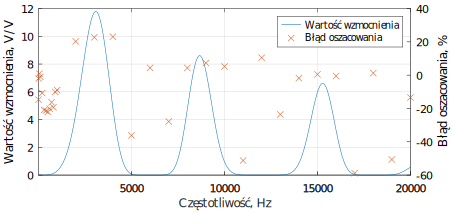
\includegraphics[scale = 0.75]{obrazki/mono_freqcomp}
\caption{Zależność wartości względnego błędu oszacowania wartości niepewności rozszerzonej \qty{24}{\numTej} wielkości wyjściowej algorytmu DWT w funkcji częstotliwości sygnału wejściowego $s(t)$, średnia wartości bezwzględnych wynosi \qty{11.74}{\percent}}
\label{fig:mono_freqcomp}
\end{center}
\end{figure}
\end{frame}

\begin{frame}{Przypadek sygnału monoharmonicznego}
\begin{itemize}
\item Niedokładne oszacowane parametrów sygnału błędu losowego $e_{s,r}(t)$ -- dokumentacja układu, widoczne gdy dominujące źródło błędów stanowią sygnały błędów losowych
\item Niewłaściwa aproksymacja charakterystyki wartości przesunięcia fazowego $\tilde{\varphi}_{s,x}(\omega)$ -- pomiary, wartość przeszacowana dla niskich wartości pulsacji
\item Pominięcie zjawiska \enquote{Jitter} -- problematyka opóźnień nie stanowiła tematyki pracy
\end{itemize}
\begin{itemize}
\item Średnia wariancja sygnału błędu wypadkowego dla analizowanego zakresu częstotliwości została oszacowana prawidłowo
\item Algorytm DWT wzmacnia/tłumi wybrane zakresy częstotliwości, stąd różnice w szacowanej/wyznaczonej wartości niepewności rozszerzonej
\item Dla sygnału poliharmonicznego wyciągnąć można podobne wnioski
\end{itemize}
\end{frame}

\newsection{Podsumowanie}{Przedstawienie najważniejszych wniosków płynących z pracy}

\begin{frame}{Wnioski}
\begin{itemize}
\item Zaproponowany model błędów może być stosowany dla torów pomiarowych wykorzystujących algorytmy transformacji falkowej
\item Zaproponowana metoda szacowania wypadkowej wartości niepewności rozszerzonej zapewnia wyniki zbliżone do uzyskiwanych metodą Monte-Carlo
\item Niska złożoność obliczeniowa umożliwia aplikację metody w czasie rzeczywistym, również w przypadku zmiany parametrów modelu błędów
\item Dokładność uzyskiwanych wyników zależy od dokładności określenia parametrów modelu błędów
\item Aby uzyskać bardziej dokładne wyniki należy przeprowadzić odpowiednie badania w celu ustalenia dokładnych parametrów modelu błędów, w szczególności dla stosowanego generatora
\end{itemize}
\end{frame}

\section*{Zakończenie}

\begin{frame}[plain]
\lastpage
\end{frame}

\end{document}
